\section{Dynamisk Programmering}
\hrulefill

\begin{itemize}
\item{Elementer af dynamisk programmering}
\item Rod-Cutting
  \begin{itemize}
  \item Køretid
  \item Optimal delstruktur
  \item Overlappende delproblemer
  \item Top-down
  \item Bottom-up
  \end{itemize}
\item Longest Common Subsequence
  \begin{itemize}
  \item Optimal delstruktur
  \item Overlappende delproblemer
  \item dynamisk programmering algoritmen
  \item Recap af de 4 trin
  \end{itemize}
\end{itemize}

\newpage
\subsection{Elementer af dynamisk programmering}
Dynamisk programmering, ligesom del og hersk, løser problemer ved at dele dem op og løse underproblemerne. En forskel er dog, at problemerne skal udvise to egenskaber, for at dynamisk programmering er praktisk at bruge: Problemet skal udvise \textbf{optimal delstruktur}, hvilket betyder at løsningen til et problem indeholder løsningen til delproblemer. Den anden egenskab et dynamisk programmering problem skal udvise er \textbf{overlappende delproblemer}, hvilket betyder at det samme delproblem skal løses flere gange for at nå frem til en løsning til det endelige problem.\\

Der er 4 trin man følger for et dynamisk programmering problem:
\begin{itemize}
\item Karakteriser en optimal løsnings struktur.
\item Rekursivt definer værdien af en optimal løsning.
\item Bestem værdien af en optimal løsning.
\item Konstruer selve den optimale løsning ud fra de løste værdier.
\end{itemize}

De første 3 trin giver værdien til en optimal løsning, mens det sidste trin er valgfrit, og giver løsningen der hører til værdien. 

\subsection{Rod-Cutting}
Man får givet en stav af længde $n$ og en liste $p_i$ med priser, således at en stav af længde $k$ har prisen $p_k$. Med en stav af længde $n$ er der $2^{n-1}$ måder at skære staven på - ved hver længde kan man enten vælge at skære, eller ikke at skære.\\
En måde at beskrive prisen man kan få for en stav er, ved at skære staven i to dele og rekursivt checke den optimale pris, og så vælge maximum af de priser
$$r_n = max(p_n, r_1 + r_{n - 1}, r_2 + r{n - 2}, ..., r_{n - 1} + r_1)$$

En lettere måde at beskrive den rekursive løsning er, at ved at vælge den maksimale pris ved at sælge en stav af længde $i$ plus den optimale pris ved en stav af $n-i$
$$r_n= max_{1 \leq i \leq n}(p_i + r_{n-i})$$

\subsubsection{Køretid}
Køretiden af den rekursive rod-cutting algoritme er $Ø(2^n)$, da den tjekker alle $2^{n-1}$ løsninger. Mere formelt kan vi se på køretiden $T(n)$ for algoritmen, hvor vi beskriver køretiden som en rekursionsligning $T(n) = 1 + \sum_{i=0}^{n-1}T(i)$, hvor 1 er kaldet for roden, det oprindelige kald til $T(n)$, og det næste led summerer over alle de rekursive kald der bliver foretaget.\\

\textbf{Bevis af køretid}\\
Vi beviser køretiden ved substitutionsmetoden, hvor base case er $T(0) = 1 + \sum_{i=0}^{0-1}T(i) = 1 = 2^0$. Vi går nu ud fra at $T(m) = 2^m$, for $m < n$.
\begin{proof}
\begin{align*}
  T(n) &= 1 + \sum_{i=0}^{n-1} T(i)\\
       &= 1 + \sum_{i=0}^{n-1} 2^i\\
       &= 1 + (2^n - 1)\\
       &= 2^n
\end{align*}
Køretiden for rod-cutting er $Ø(2^n)$.
\end{proof}

Denne køretid er ikke praktisk for store længder $n$, men heldigvis kan den forbedres ved brug af dynamisk programmering.
\subsubsection{Optimal delstruktur}
En egenskab der skal til for at kunne benytte dynamisk programmering til at løse et problem er, at problemet skal udvise optimal delstruktur. Det betyder, at løsningen til et problem indeholder løsningen til underproblemer. I tilfældet med rod-cutting algoritmen, ses det i, at når vi skal finde den optimale pris for en stav af længde $n$, skal vi finde den optimale pris for stavlængder op til $n-1$.

\subsubsection{Overlappende underproblemer}
En anden egenskab der skal gøre sig gældende for, at dynamisk programmering er praktisk at bruge er, at der skal udvises overlappende underproblemer. Overlappende underproblemer er, når det samme underproblem skal løses flere gange. I rod-cutting ses det i, at den optimale pris for at finde den optimale pris af en stavlængde $n$, skal man finde den optimale pris for stavlængden $i < n$ $2^{n-i}$ gange.

\subsubsection{Top-down}
Man kan forbedre $Ø(2^n)$ ved at bruge dynamisk programmering. I top-down bruger man et array eller en anden datastruktur til at gemme løsningen til underproblemer, så næste gang et rekursivt kald støder på det samme underproblem skal det ikke løses igen, men kan læses fra datastrukturen på konstant tid.\\
Nedenunder ses algoritmerne til memoized cut-rod. \texttt{MEMOIZED-CUT-ROD} initialiserer et array $r$, som funktionen \texttt{MEMOIZED-CUT-ROD-AUX} bruger til at gemme løsninger til delproblemer.

\begin{algorithm}[H]
  \caption{Top-down funktion bruger tabel til memoization.}
  \begin{algorithmic}[1]
    \State $p[1...n]$ er array med stavpriser for stav af længde $i=1, 2, ..., n$
    \Function{MEMOIZED-CUT-ROD}{$p, n$}
    \For{$i = 0$ \textbf{to} $n$}
    \State $r[i] = -\infty$
    \EndFor
    \State \textbf{return} MEMOIZED-CUT-ROD-AUX($p, n, r$)
    \EndFunction
  \end{algorithmic}
\end{algorithm}
\begin{algorithm}[H]
  \caption{Selve cut-rod funktionen til memoization.}
  \begin{algorithmic}[1]
    \State $p[1...n]$ er array med stavpriser for stav af længde $i=1, 2, ..., n$
    \State $r[1...n]$ er array med optimal løsning på delproblemer af cut-rod
    \Function{MEMOIZED-CUT-ROD-AUX}{$p, n, r$}
    \If{$r[n] \geq 0$}
    \State \textbf{return} $r[n]$
    \EndIf
    \If{$n==0$}
    \State $q=0$
    \Else
    \State $q = -\infty$
    \For{$i=1$ \textbf{to} $n$}
    \State $q = max(q, p[i] + $MEMOIZED-CUT-ROD-AUX$(p, n-i, r))$
    \EndFor
    \EndIf
    \State $r[n] = q$
    \State \textbf{return} $q$
    \EndFunction
  \end{algorithmic}
\end{algorithm}

\subsubsection{Bottom-up}
I bottom-up metoden starter man med at løse, som navnet hentyder, fra bunden og op. Et problem bliver ikke løst, før delproblemer, som det problem afhænger af, er blevet løst. Her er der ikke brug for en datastruktur til at gemme på løsningerne til delproblemer, da løsningen bruges umiddelbart efter den er fundet.\\

\begin{algorithm}[H]
  \caption{Selve cut-rod funktionen til memoization.}
  \begin{algorithmic}[1]
    \State $p[1...n]$ er array med stavpriser for stav af længde $i=1, 2, ..., n$
    \Function{BOTTOM-UP-CUT-ROD}{$p, n,$}
    \State $r[1...n] = $nyt array
    \State $r[0] = 0$
    \For{$j = 1$ \textbf{to} $n$}
    \State $q = -\infty$
    \For{$i = 1$ \textbf{to} $j$}
    \State $q = max(q, p[i] + r[j-i]$
    \EndFor
    \State $r[j] = q$
    \EndFor
    \State \textbf{return} $r[n]$
    \EndFunction
  \end{algorithmic}
\end{algorithm}

Både top-down og bottom-up giver en ny køretid på $\Theta(n^2))$. I bottom-up er det åbenlyst, da vi iterer over to for-loops. I top-down skyldes det at vi har et for-loop, og hver løsning bliver løst 1 gang.\\



\subsection{Longest common subsequence}
En delfølge af en følge $X$ består af elementerne fra $X$ hvor nogle er blevet udeladt. F.eks. $X= \langle 1, 2, 3, 4, 5\rangle$ kunne delfølger være $X' = {\langle 1, 2\rangle}, \langle 1, 4, 5\rangle$ etc.\\

Longest common subsequence algoritmen finder den længste delfølge som er en delfølge af to følger $X$ og $Y$.

En naiv måde at løse LCS problemet er, at sammenligne alle delfølger af $X$ med alle delfølger af $Y$.
Siden en delfølge kan tage den binære beslutning om at inddrage eller udelade et element af den oprindelige følge, er der $2^n$ delfølger, derfor giver det sig at denne metode er upraktisk.

\subsubsection{Optimal delstruktur}
For at vi kan bruge dynamisk programmering til at forbedre LCS, skal vi vise at LCS udviser optimal delstruktur, ved at en LCS af to følger indeholder LCS til "prefix" af de følger, hvor en prefix $i$ af en følge $X$ er de første $i$ elementer af $X$, således at $X_i = \langle x_1, x_2, ..., x_i\rangle$.\\

\textbf{Bevis for at optimal delstruktur af LCS}\\
\begin{theorem}
Hvis vi har to følger $X = \langle x_1, x_2, ..., x_m \rangle$ og $Y = \langle y_1, y_2, ..., y_n \rangle$, og vi har en LCS af de to følger $Z = \langle z_1, z_2, ..., z_k\rangle$.
\begin{enumerate}
\item hvis $x_m = y_n$ så $z_k = x_m = y_n \Rightarrow Z_{k-1}$ er en LCS af $X_{m-1}$ og $Y_{n-1}$
\item hvis $x_m \neq y_n$ så $z_k \neq x_m \Rightarrow Z$ er en LCS af $X_{m-1}$ og $Y$
\item hvis $x_m \neq y_n$ så $z_k \neq y_n \Rightarrow Z$ er en LCS af $X$ og $Y_{n-1}$
\end{enumerate}
\end{theorem}
Altså hvis $Z$ er en LCS af $X$ og $Y$, så må $Z_{k-1}$ være en optimal delfølge for et prefix af $X$ og $Y$. \\

Tilfælde 2 og 3 er symmetriske, hvor $X$ og $Y$ er byttet rundt.\\
\begin{proof}
Vi starter med 1. tilfælde:\\
Hvis $Z$ er en LCS, hvor $x_m = y_n$ og vi antager at $z_k \neq x_m$, så kan vi blot tilføje $x_m = y_m$ til $Z$, hvor vi så får en LCS af længde $k + 1$, hvilket er i modstrid med at $Z$ allerede var en LCS.\\
Nu har vi at $Z_{k-1}$ er en LCS af $X_{m-1}$ og $Y_{n-1}$. Lad os antage at der findes en fælles delfølge $W$ af $X_{m-1}$ og $Y_{n-1}$ som har en længde større end $k - 1$. Siden $x_m = y_n$ kan vi tilføje $x_m = y_n$ til $W$, som så får en længde $k + 1$, hvilket er i modstrid med antagelsen at $Z$ var en LCS.\\
Altså, hvis $x_m = y_n$, så er $Z_{k-1}$ en LCS af $X_{m-1}$ og $Y_{n-1}$.\\

2. tilfælde:\\
Hvis $x_m \neq y_m$ og vi antager at $z_k \neq x_m$, så må $Z$ være en LCS af $X_{m-1}$ og $Y$.\\
Hvis vi antager at der findes en fælles delfølge $W$ af $X_{m-1}$ og $Y$, som har længde større end $k$, så ville $W$ også være en fælles delfølge af $X_m$ og $Y$, siden vi fra tilfælde 1 ved at vi ikke kan tilføje $X_m=y_n$. Dette er i modstrid med at $Z$ er en LCS af $X$ og $Y$, siden $W$ har længde større end $k$\\
Altså, hvis halerne i $X$ og $Y$ ikke er ens, men $z_k=y_n$, så fjerner vi $i$ elementer halen af $X$, indtil vi finder et fælles element. $Z_{k-1}$ er så en delfølge af $X_{m-i}$ og $Y_{n-1}$\\

3. tilfælde er symmetrisk med 2. tilfælde, med $X$ og $Y$ byttet rundt.
\end{proof}

\subsubsection{Overlappende delproblemer}
LCS algoritmen udviser også overlappende delproblemer. Vi viste før, at hvis $x_m \neq y_n$, så skal vi løse to delproblemer; at finde en LCS til $X_{m-1}$ og $Y$, og finde en LCS til $X$ og $Y_{n-1}$.
\begin{equation}
  c[i,j] = 
  \begin{cases}
    0 & \text{hvis } i=0 \text{ or } j=0\\
    c[i-1, j-1] & \text{hvis } i,j > 0 \text{ og } x_i = y_j\\
    max(c[i-1, j], c[i, j-1]) & \text{hvis } i,j > 0 \text{ og } x_i \neq y_j
  \end{cases}
\end{equation}

Hver af disse to delproblemer skal så løse tilsvarende delproblemer. Et træ for de overlappende delproblemer kan ses her:
\begin{figure}[h!]
  \caption{Overlappende delproblemer. Knuderne viser prefix $m$ for $X$, og $n$ for $Y$.}
\begin{center}
        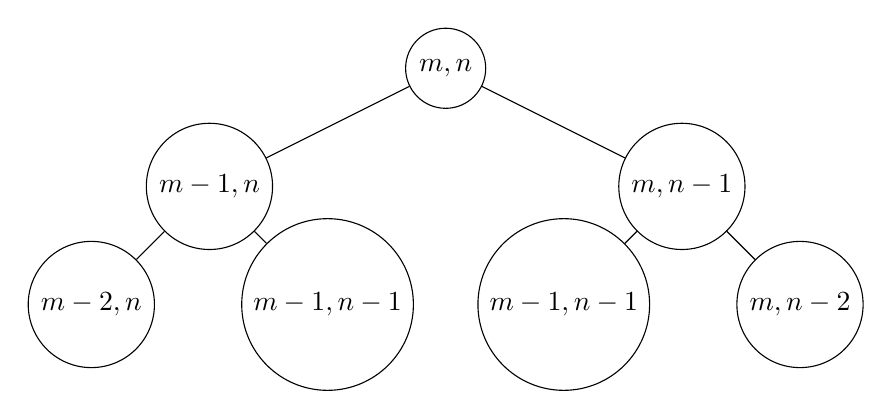
\begin{tikzpicture}[every node/.style = {shape=circle, draw, align=center, minimum width= 1cm}, level distance=1.5cm,
          level 1/.style={sibling distance=6cm},
          level 2/.style={sibling distance=3cm},
          level 3/.style={sibling distance=1.5cm},
          emph/.style={edge from parent/.style={dashed,draw}}]
          \node(A) at (0, 0) {$m, n$}
          child { node {$m - 1, n$}
            child { node {$m - 2, n$} }
            child { node {$m - 1, n - 1$}}}
          child { node {$m, n - 1$}
            child { node {$m - 1, n - 1$} }
            child { node {$m, n - 2$} }};
        \end{tikzpicture}
        $$\vdots$$
\end{center}
\end{figure}

\subsubsection{Dynamisk programmering algoritmen}
Hvis vi bruger dynamisk programmering til at gemme løsninger til delproblemerne kan vi se, at vi skal løse $\Theta(mn)$ unikke delproblemer, hvilket også giver køretiden $Ø(mn)$. Løsningen til LCS problemet kan udregnes ved ligning (1), hvor $c$ arrayet indeholder alle delproblemerne. For at konstruere selve følgen, skal vi også gemme værdien i hver af de to følger $X$ og $Y$ i et array, når $x_i = y_j$.

\subsubsection{Recap af de 4 trin}
De fire trin der hører til at løse LCS problemet med dynamisk programmering er:
\begin{itemize}
\item Vi bestemte hvordan strukturen for en LCS var, ved at vise optimal delstruktur.
\item Derefter bestemte vi rekursivt hvordan vi skulle finde den optimale løsning, og vi så at problemet udviste overlappende delproblemer.
\item Vi bruger ligning (1) til at beskrive en algoritme der returnerer et 2-dimensionelt array $c$ hvor $c[m,n]$ indeholder længden af LCS'en til $X_m$ og $Y_n$\\
\item Valgfrit kan algoritmen også returnere et 2-dimensionelt array $b$ der viser hvordan vi kan konstruere et LCS.
\end{itemize}
